\chapter{Domain Decomposition}

\section{Introduction}

\index{domain decomposition}
Domain decomposition methods are based on decomposition of the original domain
where a problem is solved into several smaller subdomains. This chapter deals
only with decomposition of the mesh, which is also called mesh partitioning,
and description of submeshes (meshes defined on subdomains).
Numerical methods connected with the domain decomposition are described in ??.

Domain decomposition methods are especially popular in connection with
parallel computers because each subdomain can be elaborated by one processor
of parallel \index{parallel computer} computer. Decomposition of the original
problem and the use of parallel computer enable to solve large problems
(problems with greater number of degrees of freedom) or reduce computational
time. From this point of view, any large problem can be decomposed and solved
in parallel. Application of parallel computer and domain decomposition method
to arbitrary small problems which are solvable without difficulties on
single-processor computer is unnecessary.

Sequential (one-processor) implementation of domain decomposition methods
is useful as well because it may save memory and time. The reason is that
the sum of sizes of subdomain matrices (numbers of stored matrix entries)
may be, and usually is, smaller than the size of the matrix of the original
problem. Additional advantage of the sequential implementation is the simple
use of debugger which may save a lot of time.

Domain decomposition methods are useful without respect of the size for some
problems where explicitly two or more subdomains are recognised. Examples of
such problems are \index{contact problem}\index{problem!of contact} contact
of two or more bodies, interaction of composite
matrix \index{matrix-fibre interaction}
and fibres or any reinforcement or transport 
processes \index{transport process}
in two connected domains created by different materials. In such case,
decomposition of the problem solved is natural and application of the
domain decomposition method is useful and usually efficient.


\section{Partitioned Mesh Generation}

As was stated before, domain decomposition methods lead to a set of subdomains.
The finite element method is based on a mesh, in the case of decomposed domain
on a set of meshes. Generally, there are two types of meshes on subdomains:
\begin{itemize}
\item conforming meshes,
\item nonconforming meshes.
\end{itemize}
\index{conforming mesh}\index{mesh!conforming}
\index{nonconforming mesh}\index{mesh!nonconforming}

The conforming meshes are meshes where intersection of two elements is the empty set,
a node, a whole edge or a whole surface. The conforming meshes can be denoted as the
classical ones. All other meshes are denoted as nonconforming meshes and they require
a special treatment in order to enforce continuity. An example of such special treatment
is the mortar element \index{mortar element method}\index{method!mortar} method.

A partitioned mesh can be obtained by:
\begin{itemize}
\item partitioning of a whole mesh,
\item mesh generation on particular subdomains.
\end{itemize}
There are many algorithms for \index{mesh partitioning} mesh partitioning. For
example, the greedy \index{greedy algorithm}\index{algorithm!partitioning!greedy} algorithm,
the nested \index{nested dissection}\index{algorithm!partitioning!nested dissection} disssection \cite{Meurant}.
Advantage of mesh partitioning is, that conforming mesh before partitioning results
in conforming meshes which are simpler for manipulation with them. Mesh generation
on particular subdomains leads generally to nonconforming meshes. The conforming
meshes require a special mesh generation which communicates among subdomains.

\section{Definitions of Basic Notation}

\noindent
{\bf Definition.}
The internal node \index{node!internal}\index{internal node} is a node which belongs just to one subdomain.

Node lying on the boundary of the problem which belongs only to one subdomain are also denoted as internal
node. Such nodes are not important from the point of domain decomposition methods because there is no need
for continuity enforcement.

\noindent
{\bf Definition.}
The interface node \index{node!interface}\index{interface node} is a node which belongs to at least two subdomains.

The interface node is called sometimes the boundary node \index{boundary node}\index{node!boundary}
because it is located at the boundary of subdomain which was created by decomposition.
The reason for this ambiguity stems from the fact, that
the internal nodes have index $i$ and it is not clear whether $i$ denotes internal or interface. The boundary
(interface) nodes are indicated by $b$.

\noindent
{\bf Definition.}
The corner node \index{node!corner}\index{corner node} is an interface node which is in a corner in the case
of rectangular subdomains.




\noindent
{\bf Definition.}
Ordering of nodes or degrees of freedom on the original mesh which covers undecomposed domain is called
global \index{global ordering}\index{ordering!global} ordering.

\noindent
The global ordering is identical with ordering used in the classical sequential (one-processor) computations.
Each node or DOF has its unique number. Example of the global ordering of nodes is depicted in figure \ref{figmeshglobord}.

\begin{figure}[h]
\begin{center}
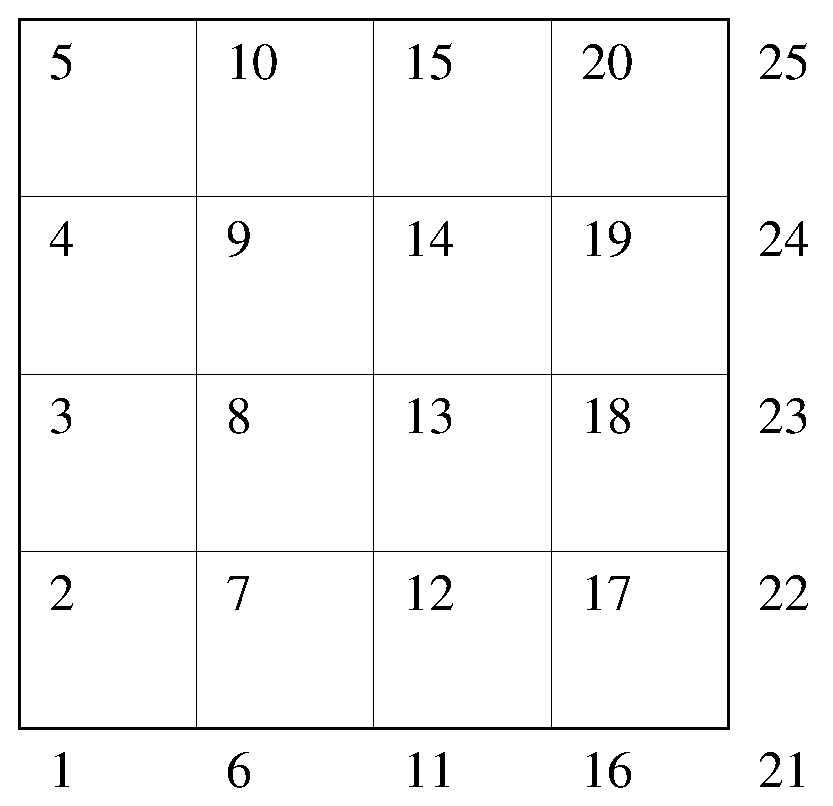
\includegraphics[width=80mm]{FIG/meshglobord.eps}
\caption{Mesh on the original domain. Global ordering.}
\label{figmeshglobord}
\end{center}
\end{figure}

\noindent
{\bf Definition.}
Ordering of nodes or degrees of freedom on particular subdomain which starts from one is called
local \index{local ordering}\index{ordering!local} ordering.

\noindent
The local ordering on particular subdomain looks like the classical ordering of nodes or DOFs on domain.
The local oredring is independent on local orderings on other subdomains. 
Example of the global ordering of nodes is depicted in figure \ref{figmeshlocord}.

\begin{figure}[h]
\begin{center}
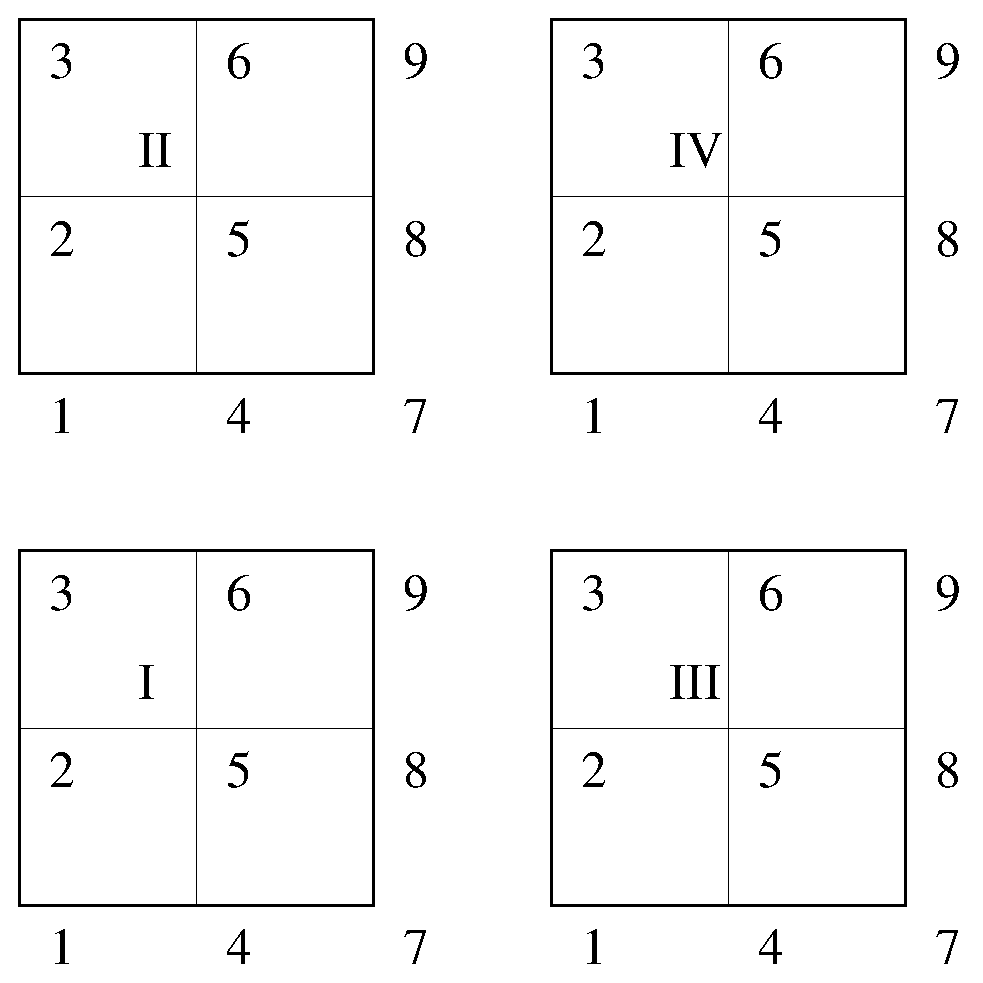
\includegraphics[width=80mm]{FIG/meshlocord.eps}
\caption{Meshes on subdomains obtained by partitioning. Local ordering.}
\label{figmeshlocord}
\end{center}
\end{figure}

\noindent
{\bf Definition.}
Ordering of nodes or degrees of freedom on particular subdomain which is continuous from the first
to the last subdomain is called
global \index{global glued ordering}\index{ordering!global glued} glued ordering.
\label{globgluedorder}

\noindent
The global glued ordering is different from the global ordering because the interface nodes
have at least two different numbers coming from subdomains which share them. The global glued
ordering can be obtained by gluing of local orderings on subdomains where the local numbers
are shifted with respect to the largest number on previous subdomain.
Example of the global glued ordering of nodes is depicted in figure \ref{figmeshglobgluedord}.


\begin{figure}[h]
\begin{center}
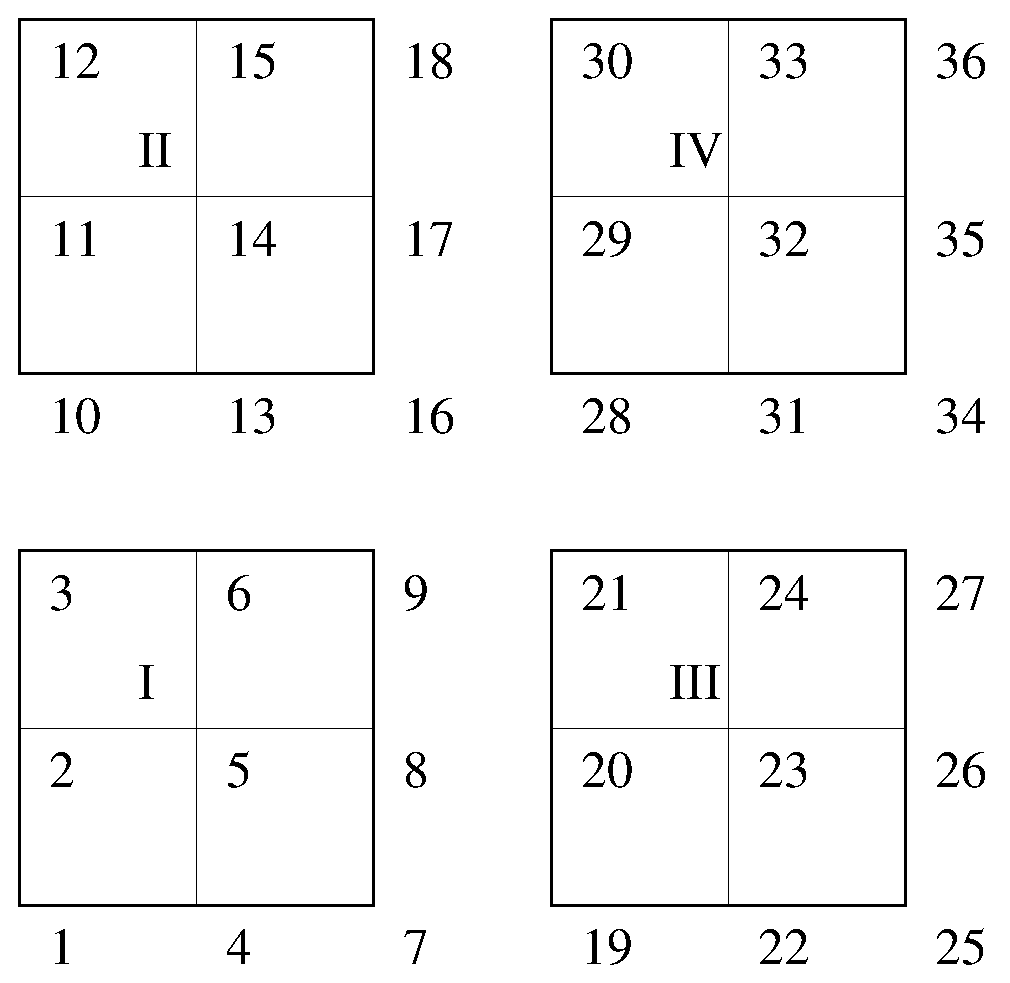
\includegraphics[width=80mm]{FIG/meshglobgluedord.eps}
\caption{Meshes on subdomains obtained by gluing. Global glued ordering.}
\label{figmeshglobgluedord}
\end{center}
\end{figure}

\noindent
{\bf Definition.}
Ordering of nodes or degrees of freedom on the original mesh which covers undecomposed domain is called
negative global \index{negative global ordering}\index{ordering!negative global} ordering if
the interface nodes have their numbers multiplied by minus one.

\noindent
The negative global ordering simplifies searching for the interface nodes and DOFs.
Example of the negative global ordering of nodes is depicted in figure \ref{figmeshnegglobord}.

\begin{figure}[h]
\begin{center}
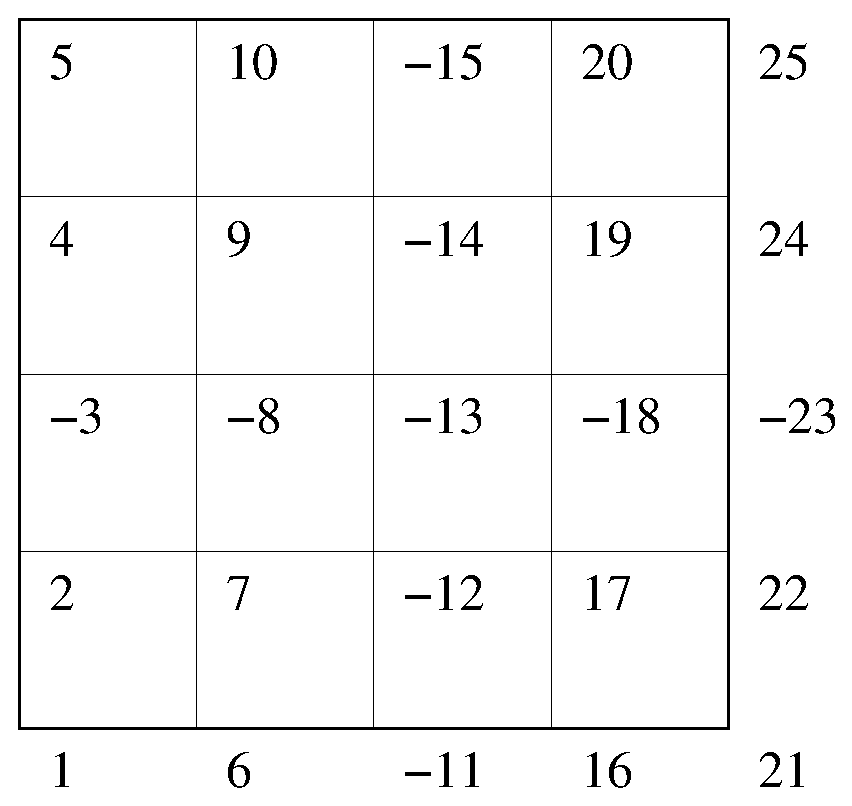
\includegraphics[width=80mm]{FIG/meshnegglobord.eps}
\caption{Mesh on the original domain. Negative global ordering.}
\label{figmeshnegglobord}
\end{center}
\end{figure}

\noindent
{\bf Definition.}
Ordering of interface nodes or degrees of freedom only on the whole problem is called
coarse \index{coarse ordering}\index{ordering!coarse} ordering.

\noindent
The coarse ordering is important in domain decomposition methods beacuse it assures
compatibility among subdomains.
Example of the coarse ordering of nodes is depicted in figure \ref{figmeshcoarseord}.

\begin{figure}[h]
\begin{center}
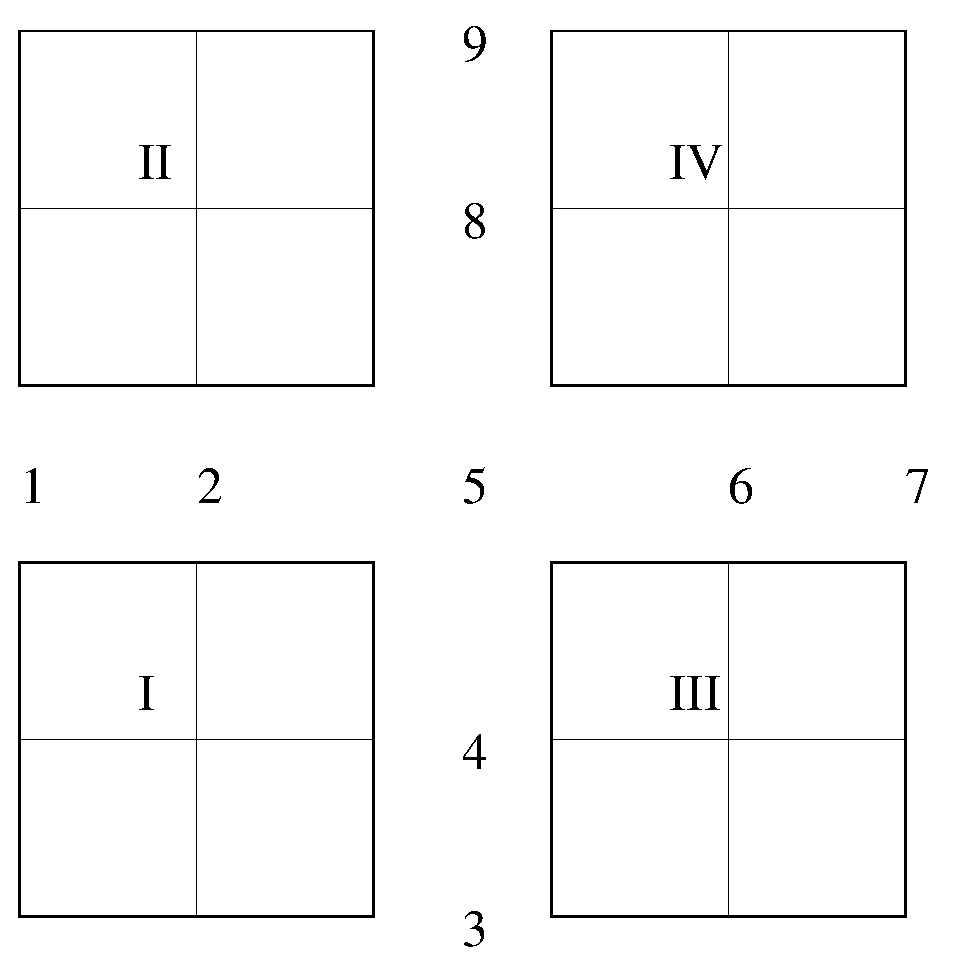
\includegraphics[width=80mm]{FIG/meshcoarseord.eps}
\caption{Coarse ordering.}
\label{figmeshcoarseord}
\end{center}
\end{figure}


Domain decomposition methods contain at least two levels of computation. The local
level deals with subdomains while the coarse level deals with the interface.
Notation coarse follows from the fact, that the interface is similar to a coarse
mesh which can be obtained by elimination of internal nodes or DOFs.
Two orderings of nodes and DOFs are used. The local ordering is used on the local
level and the coarse ordering is used on the coarse level.

The crucial point is correct connection between local and coarse ordering.
The global ordering and the global glued ordering are auxiliary tools for
establishing of the connection between local and coarse ordering.


Connection between local and coarse ordering is created with the help of
\index{\sf ltg}\index{array!{\sf ltg}} array ltg.
Format of the array ltg depends on the variable meshdescription (\ref{sectmeshdescription}).
\index{\sf meshdescription}\index{variable!{\sf meshdescription}}


{\tt
1 2 3 6 7 8 11 12 13
\newline
3 4 5 8 9 10 13 14 15
\newline
11 12 13 16 17 18 21 22 23
\newline
13 14 15 18 19 20 23 24 25
}

{\tt
0 0 1 0 0 2 3 4 5
\newline
1 0 0 2 0 0 5 8 9
\newline
3 4 5 0 0 6 0 0 7
\newline
5 8 9 6 0 0 7 0 0
}


{\tt
1 2 -3 6 7 -8 -11 -12 -13
\newline
-3 4 5 -8 9 10 -13 -14 -15
\newline
-11 -12 -13 16 17 -18 21 22 -23
\newline
-13 -14 -15 -18 19 20 -23 24 25
}


%%%%%%%%%%%%%%%%%%%%%%%%%%%%%%%%%%%%%%%%%%%%%%%%%%%%%%%%
%%%%%%%%%%%%%%%%%%%%%%%%%%%%%%%%%%%%%%%%%%%%%%%%%%%%%%%%
%%%%%%%%%%%%%%%%%%%%%%%%%%%%%%%%%%%%%%%%%%%%%%%%%%%%%%%%
%%%%%%%%%%%%%%%%%%%%%%%%%%%%%%%%%%%%%%%%%%%%%%%%%%%%%%%%
\section{Implementation}

{\bf variant: boundary nodes}

\begin{itemize}
\item
mefel\_init (int argc, char *argv[],stochdriver *stochd) (mefelinit.cpp)

\item
$\Uparrow$ read (XFILE *in) (mechtop.cpp)

\item
$\Uparrow$ Gtm--$>$read\_seq\_top (Mp--$>$ssle--$>$feti.ns,in) --- creates object stop of the class seqtop,

\item
$\Uparrow$ stop--$>$read\_ltg (XFILE *in) (seqtop.cpp) --- allocates and reads array ltg,
local to global correspondence,
ltg[i][j]=k - the j-th node on the i-th subdomain has coarse number k,
k$>$-1 - number of coarse unknown,
k=-1 - the node is internal node,
\newline
$\Uparrow$ stop--$>$read\_nnsd (in); --- allocates and reads array nnsd,
array containing number of nodes on subdomains,
it contains nproc components,
nnsd[i]=j - j nodes are defined on the i-th subdomain,


\item 
gt--$>$stop--$>$compute\_multiplicity (out); 
\newline
array nbnd is allocated, 
array containing list of numbers of boundary/interface nodes on subdomains,
it contains ns components,
nbnd[i]=j - the i-th domain contains j boundary/interface nodes,
\newline
multip is allocated, 
array containing number of subdomains which each boundary/interface node belongs to,
it contains tnnp or tnbn components, it depends on the type of mesh description,
multip[i]=j - the i-th node belongs to j subdomains,
\newline
nodmultip is allocated,
array containing number of subdomains which share the nodes,
it contains ns, nnsd[i] components,
nodmultip[i][j]=k - the j-th node of the i-th subdomain belongs to k subdomains,
\newline
tnbn - total number of interface (boundary) nodes is computed, 


\item
gt--$>$stop--$>$find\_boundary\_nodes (out);
\newline
lgnbn is allocated, 
array containing list of global numbers of interface nodes,
lgnbn[i][j]=k - the j-th interface node on the i-th subdomain has global number k,
\newline
lnbn is allocated,
array containing numbers of boundary nodes,
it contains ns, nbnd[i] components,
lnbn[i][j]=k - the j-th boundary node on the i-th subdomain has local number k,
\newline
nind is allocated,
array containing list of numbers of internal nodes on subdomains,
it contains ns components,
nind[i]=j - the i-th domain contains j internal nodes,
\newline
lnin is allocated,
array containing numbers of internal nodes,
it contains ns, nind[i] components,
lnin[i][j]=k - the j-th internal node on the i-th subdomain has local number k,


\item
gt--$>$stop--$>$rewrite\_ltg (); --- array ltg is rewritten,

\item
object selnodfeti of the class seqselnodes (feti.ns,gt--$>$stop--$>$nnsd,fetinodes,gt--$>$stop--$>$md,out,1); is allocated,
\newline
nsndom is allocated,
numbers of selected nodes,
nsndom[i]=j - there are j selected nodes on the i-th subdomain,
\newline
lsnl is allocated,
list of selected nodes - local numbers,
lsnl[i][j]=k - the j-th selected node on the i-th subdomain has local number k,
lsnl contains ns,nsn[i] components,
\newline
lsng is allocated,
list of selected nodes - global numbers,
lsng[i][j]=k - the j-th selected node on the j-th subdomain has global/coarse number k,
lsng contains ns, nsn[i] components,


\item
selnodfeti--$>$nodes\_on\_master (gt--$>$nn,out);
\newline
gnn is allocated,
group node numbers (see partop.h),
gnn[i][j]=k - the j-th selected node on the i-th subdomain has group number k,
\newline
tnsn - total number of selected nodes is computed,

\item
selnodfeti--$>$node\_multiplicity (out);
\newline
nodmultip is allocated,
node multiplicity,
nodmultip[i]=j - the i-th selected node is shared by j subdomains,
it contains tnsn components,

\item
selnodfeti--$>$number\_all\_dofs (gt,out);
\newline
ndofdom is allocated,
array of numbers of DOFs on subdomains,
it contains prescribed values before code number generation,
after code number generation, only unknown (unconstrained DOFs) are taken into account,
array is rewritten in the function schur\_ordering,
ndofdom[i]=j - the i-th subdomain contains j DOFs,

\item
selnodfeti--$>$ndofn\_on\_master (gt,out);
\newline
ndofnmas is allocated,
array of DOFs at selected nodes,
ndofnmas[i][j]=k - the j-th node on the i-th subdomain contains k DOFs,

\item
selnodfeti--$>$dof\_indicators (gt,out);
\newline
dofmas is allocated,
array of DOFs or indicators on master,
dofmas[i][j][k]=l - the k-th DOF at the j-th selected node on the i-th subdomain has value l,


\item
selnodfeti--$>$group\_local\_nodes (out);
\newline
ljn is allocated,
list of joint nodes to selected nodes assumed as coarse nodes,
ljn[i][j]=k - the j-th node connected to the i-th coarse node has local number k,
ljn contains tnsn rows and nodmultip columns,
\newline
lsn is allocated,
list of subdomain numbers which contain connected nodes to coarse nodes,
lsn[i][j]=k - the j-th node connected to the i-th coarse node belongs to the k-th subdomain,
lsn contains tnsn rows and nodmultip columns,


\item
selnodfeti--$>$dof\_feti (out);
\newline
ndofnsn is allocated,
array of numbers of DOFs for selected nodes,
ndofnsn[i]=j - the i-th selected node (in group ordering) has j DOFs,
it contains tnsn components,
\newline
doffeti is allocated,
code numbers / indicators for FETI method,
doffeti[i][j][k]=l - the k-th DOF on the j-th connected node to the i-th coarse node has code number / indicator l,

\item
selnodfeti--$>$number\_contrib (out);
\newline
ndofdom is allocated,
array of numbers of DOFs on subdomains,
it contains prescribed values before code number generation,
after code number generation, only unknown (unconstrained DOFs) are taken into account,
array is rewritten in the function schur\_ordering,
ndofdom[i]=j - the i-th subdomain contains j DOFs,
\newline
ncndom is allocated,
number of contributing nodes in the FETI method,
ncndom[i]=j - the i-th subdomain contributes to the coarse problem by j nodes,

\item
selnodfeti--$>$contrib\_dofs (gt,out);
\newline
ndofdom
array of numbers of DOFs on subdomains,
it contains prescribed values before code number generation,
after code number generation, only unknown (unconstrained DOFs) are taken into account,
array is rewritten in the function schur\_ordering,
ndofdom[i]=j - the i-th subdomain contains j DOFs,
\newline
ldof
list of code numbers which contribute to the coarse problem,
ldof[i][j]=k - the j-th DOF on the i-th subdomain has local code number k,
\newline
cndom
code numbers on master,
cndom[i][j]=k - the j-th DOF on the i-th subdomain has group code number k,


\item
feti.initiate (selnodfeti,gt,out);
\newline
ncdofd
array of numbers of unknowns (DOFs) contributing to the coarse problem
ncdofd contains nproc components
ncdofd[i]=j - the i-th subdomains contributes to coarse problem by j contributions
\newline
edofs is allocated
array containing code numbers contributing to the coarse problem
extracted values from subdomains to the coarse problem
edofs[i][j]=k - the j-th components contributing to the coarse problem from the i-th subdomains has number k
\newline
ccn
array of coarse code numbers
it contains tnbn rows and ncdofd[i] columns
ccn[i][j]=k - the j-th contribution from the i-th subdomain goes to the k-th coarse unknown

\item
feti.assemble\_subdom\_unknowns (gt,out);
\newline
nsid
node-subdomain correspondence
nsid[i]=j - the i-th node belongs to the j-th subdomain
\newline
ndofdom
numbers of DOFs on subdomains
ndofdom[i]=j - the i-th subdomain contains j DOFs
\newline
cndom
list of DOFs on subdomains
cndom[i][j]=k - the j-th DOF on the i-th subdomain has number k


\end{itemize}

{\bf variant: boundary nodes}
\begin{itemize}
\item
mefel\_init (int argc, char *argv[],stochdriver *stochd) (mefelinit.cpp)

\item
$\Uparrow$ read (XFILE *in) (mechtop.cpp)

\item
$\Uparrow$ Gtm--$>$read\_seq\_top (Mp--$>$ssle--$>$feti.ns,in) --- creates object stop of the class seqtop,

\item
mefel\_init (mefelinit.cpp) $=>$ Mt--$>$read (mechtop.cpp) $=>$ Gtm--$>$read\_seq\_top (gtopology.cpp) $=>$ stop--$>$read\_nnsd (in); (seqtop.cpp) --- allocates and reads array nnsd,
array containing number of nodes on subdomains,
it contains nproc components,
nnsd[i]=j - j nodes are defined on the i-th subdomain,
\newline
$\Uparrow$ stop--$>$read\_ltg (XFILE *in) (seqtop.cpp) --- allocates and reads array ltg,
local to global correspondence,
ltg[i][j]=k - the j-th node on the i-th subdomain has coarse number k,
k$>$-1 - number of coarse unknown,
k=-1 - the node is internal node,

\end{itemize}

%%%%%%%%%%%%%%%%%%%%%%%%%%%%%%%%%%%%%%%%%%%%%%%%%%%%%%%%%%%%%%%%%%%%%%%%
%%%%%%%%%%%%%%%%%%%%%%%%%%%%%%%%%%%%%%%%%%%%%%%%%%%%%%%%%%%%%%%%%%%%%%%%
%%%%%%%%%%%%%%%%%%%%%%%%%%%%%%%%%%%%%%%%%%%%%%%%%%%%%%%%%%%%%%%%%%%%%%%%
%%%%%%%%%%%%%%%%%%%%%%%%%%%%%%%%%%%%%%%%%%%%%%%%%%%%%%%%%%%%%%%%%%%%%%%%
\section{Sequential execution of domain decomposition algorithms}

\begin{itemize}
\item
finite element mesh in the JKTK format has to be prepared, the file with mesh may be
named mesh.aux
\item
input file to METIS decomposer has to be prepared, the code metisprep may be used,
{\tt metisprep mesh.aux mesh.txt}
\item
the mesh has to be decomposed into n submeshes, e.g.
{\tt partdmesh mesh.txt n}, file mesh.txt.epart.n will be created,
\item
one file with all submeshes in the JKTK format has to be generated,
{\tt seqdd mesh.aux mesh.txt.epart.n mesh.top n}, the file mesh.top is in the
JKTK format which is extended at the end by the list of numbers of nodes on 
subdomains and for each subdomain there is list of global node numbers
\end{itemize}

%%%%%%%%%%%%%%%%%%%%%%%%%%%%%%%%%%%%%%%%%%%%%%%%%%%%%%%%%%%%%%%%%%%%%%%%
%%%%%%%%%%%%%%%%%%%%%%%%%%%%%%%%%%%%%%%%%%%%%%%%%%%%%%%%%%%%%%%%%%%%%%%%
%%%%%%%%%%%%%%%%%%%%%%%%%%%%%%%%%%%%%%%%%%%%%%%%%%%%%%%%%%%%%%%%%%%%%%%%
%%%%%%%%%%%%%%%%%%%%%%%%%%%%%%%%%%%%%%%%%%%%%%%%%%%%%%%%%%%%%%%%%%%%%%%%
\section{Automatic Subdomains Detection}

Automatic subdomain detection could be used only for conforming meshes and
twodimensional problems at this time.
Automatic subdomain detection is used e.g. in problems hemivariational inequalities.

It is based on global glued ordering (see \ref{globgluedorder}).

gtopology::auto\_subdom\_detection

\begin{itemize}
\item
gtopology::edges --- function assembles list of adjacent nodes to nodes (adjacnodes),
array of objects gedges of the class gedge are allocated and initiated
\item
gtopology::edgenode\_sorting () --- function sorts first and last nodes on edges
\item
gtopology::prev\_next\_edges --- function searches for previous and next edges for each edge
\item
gtopology::edge\_series () --- function searches for series of edges
\item
gtopology::edge\_elem --- function assignes numbers of element to edges
\item
gtopology::edge\_dirvect () --- function computes direction vectors of edges
\item
gtopology::edge\_normvect () --- function computes direction vectors of edges
\item
gtopology::normvectorient () --- function checkes orientation of normal vectors
\item
gtopology::create\_ltg (FILE *out) --- 
\end{itemize}


%%%%%%%%%%%%%%%%%%%%%%%%%%%%%%%%%%%%%%%%%%%%%%%%%%%%%%%%%%%%%%%%%%%%%%%%
%%%%%%%%%%%%%%%%%%%%%%%%%%%%%%%%%%%%%%%%%%%%%%%%%%%%%%%%%%%%%%%%%%%%%%%%
%%%%%%%%%%%%%%%%%%%%%%%%%%%%%%%%%%%%%%%%%%%%%%%%%%%%%%%%%%%%%%%%%%%%%%%%
%%%%%%%%%%%%%%%%%%%%%%%%%%%%%%%%%%%%%%%%%%%%%%%%%%%%%%%%%%%%%%%%%%%%%%%%
\section{Sequential Schur Complement Method}

nnsd - numbers of nodes on subdomains
9 9 9 9

ltg 

 1  2  3  6  7  8 11 12 13

11 12 13 16 17 18 21 22 23

 3  4  5  8  9 10 13 14 15

13 14 15 18 19 20 23 24 25

tnnp=25

amultip - number of subdomains which each node belongs to
 1 1 2 1 1 1 1 2 1 1 2 2 4 2 2 1 1 2 1 1 1 1 2 1 1

tnbn=9

nbnd  - numbers of boundary/interface nodes on subdomains

5 5 5 5

nind - numbers of internal nodes on subdomains

4 4 4 4

nodmultip - 

 1 1 2 1 1 2 2 2 4

 2 2 4 1 1 2 1 1 2

 2 1 1 2 1 1 4 2 2

 4 2 2 2 1 1 2 1 1


lnbn - local numbers of interface/boundary nodes

 3 6 7 8 9

 1 2 3 6 9

 1 4 7 8 9

 1 2 3 4 7

lnbn - local numbers of internal nodes

 1 2 4 5

 4 5 7 8

 2 3 5 6

 5 6 8 9


ggnbn - global glued numbers of interface/boundary nodes on subdomain


 3 6 7 8 9

10 11 12 15 18

19 22 25 26 27

28 29 30 31 34


ggnin - global glued numbers of internal nodes on subdomain

 1 2 4 5

13 14 16 17

20 21 23 24 

32 33 35 36

icnbn - coarse numbers of interface/boundary nodes on subdomain


 1 2 3 4 5

 3 4 5 8 9

 1 2 5 6 7

 5 6 7 8 9

icmultip - coarse-local correspondence 

 coarse node      0, number of nodes  2

 coarse node      1, number of nodes  2

 coarse node      2, number of nodes  2

 coarse node      3, number of nodes  2

 coarse node      4, number of nodes  4

 coarse node      5, number of nodes  2

 coarse node      6, number of nodes  2

 coarse node      7, number of nodes  2

 coarse node      8, number of nodes  2


ggnbncn - global glued numbers of boundary/interface nodes

 coarse node      0   ggn      3, sub.   1   ggn     19, sub.   3

 coarse node      1   ggn      6, sub.   1   ggn     22, sub.   3

 coarse node      2   ggn      7, sub.   1   ggn     10, sub.   2

 coarse node      3   ggn      8, sub.   1   ggn     11, sub.   2

 coarse node      4   ggn      9, sub.   1   ggn     12, sub.   2   ggn     25, sub.   3   ggn     28, sub.   4

 coarse node      5   ggn     26, sub.   3   ggn     29, sub.   4

 coarse node      6   ggn     27, sub.   3   ggn     30, sub.   4

 coarse node      7   ggn     15, sub.   2   ggn     31, sub.   4

 coarse node      8   ggn     18, sub.   2   ggn     34, sub.   4


nsndom - numbers of slected nodes on subdomains
5 5 5 5

ggnsn - global glued numbers of selected nodes

  3  6  7  8  9

 10 11 12 15 18

 19 22 25 26 27

 28 29 30 31 34

snndofdom - numbers of DOFs on subdomains

10 10 10 10

snndofnmas - numbers of DOFs on selected nodes

2 2 2 2 2

2 2 2 2 2

2 2 2 2 2

2 2 2 2 2

sndofmas - DOFs indicators on master

  0  0
  1  0
  1  0
  1  0
  1  0

  1  0
  1  0
  1  0
  1  0
  1  0

  0  0
  1  0
  1  0
  1  0
  1  0

  1  0
  1  0
  1  0
  1  0
  1  0

tndofsn=8

cndom - code numbers of Schur ordering

1 2 3 4

2 3 4 7 8

1 4 5 6

4 5 6 7 8

ndofdom - number of DOFs on subdomains 
6 9 6 9

cndom - array of code numbers of DOFs on subdomains 

 1 2 13 14 15 16

 3 4 5 6 17 18 19 20 21

 7 8 22 23 24 25

 9 10 11 12 26 27 28 29 30


adr in skyline

 0 1 3 5 9 14 19

 0 1 3 6 10 15 21 27 34 42

 0 1 3 6 10 15 21

 0 1 3 6 10 15 21 28 36 45


%%%%%%%%%%%%%%%%%%%%%%%%%%%%%%%%%%%%%%%%%%%%%%%%%%%%%%%%%%%%%%%%%%%%%%%%
%%%%%%%%%%%%%%%%%%%%%%%%%%%%%%%%%%%%%%%%%%%%%%%%%%%%%%%%%%%%%%%%%%%%%%%%
%%%%%%%%%%%%%%%%%%%%%%%%%%%%%%%%%%%%%%%%%%%%%%%%%%%%%%%%%%%%%%%%%%%%%%%%
%%%%%%%%%%%%%%%%%%%%%%%%%%%%%%%%%%%%%%%%%%%%%%%%%%%%%%%%%%%%%%%%%%%%%%%%
\section{Sequential FETI Method}
12. 7. 2012

Mp--$>$ssle--$>$prepare\_data (Ndofm,Gtm,Out); in mefelinit.cpp

\hspace{10mm} top--$>$stop--$>$coarse\_local\_map (top,out);

\hspace{20mm}  seqtop::compute\_multiplicity (top,out);

\hspace{30mm}  seqtop::assemble\_multip (out);

\hspace{30mm}  seqtop::coupled\_dofs (top,out);

\hspace{30mm}  seqtop::assemble\_nbnd\_nind (out);

\hspace{30mm}  seqtop::assemble\_nodmultip (out);

\hspace{30mm}  seqtop::assemble\_dofind (top,out);

\hspace{20mm}  seqtop::node\_local\_numbers (out);

\hspace{20mm}  seqtop::node\_global\_glued\_numbers (out);

\hspace{20mm}  seqtop::node\_coarse\_numbers (out);

\hspace{20mm}  seqtop::node\_coarse\_global\_glued\_map (out);

\hspace{20mm}  seqtop::node\_coarse\_local\_map (out);

\hspace{10mm}  ndof[0]=selnodfeti--$>$prepare\_feti (feti.fetiimpl,top,out);

\hspace{20mm}  seqselnodes::define\_feti\_implementation (fi);

\hspace{20mm}  seqselnodes::node\_coarse\_numbers (out);

\hspace{20mm}  seqselnodes::number\_contrib\_dofs (top,out);

\hspace{20mm}  seqselnodes::dof\_feti (top,out);

\hspace{20mm}  seqselnodes::top--$>$cngen=1;

\hspace{20mm}  seqselnodes::ndof = top--$>$codenum\_generation (out);

\hspace{20mm}  seqselnodes::contrib\_dofs\_ln (top,out);

\hspace{20mm}  seqselnodes::contrib\_dofs\_cn (out);

\hspace{10mm}   feti.initiate (selnodfeti,top,out);

\hspace{10mm} feti.assemble\_subdom\_unknowns (top,out);

\noindent
{\color{red} void seqtop::assemble\_multip (FILE *out)}
the function assembles the array {\sf bmultip} or {\sf amultip},
the function computes the variables {\sf tnnp} or {\sf tnbn}.

\noindent
{\color{red} void seqtop::coupled\_dofs (gtopology *top,FILE *out)}
the function searches for coupled DOFs which are shared by interfaces
the number of coupled DOFs on interfaces {\sf ncdof} is determined
if {\sf ncdof}$>0$, arrays {\sf coupdofmas} and {\sf coupdof}
are allocated and assmebled

\noindent
{\color{red} void seqtop::update\_multip (gtopology *top,FILE *out)}
the function updates node multiplicity,
the attributes the total number of boundary nodes {\sf tnbn} and
the total number of nodes in problem (if possible, this number cannot be
obtained in the case of md=bound\_nodes) {\sf tnnp},
array {\sf amultip} array of all node multiplicity, it is assembled if md=all\_nodes
array {\sf bmultip} array of interface/boundary node multiplicity, it is assembled if md=bound\_nodes
array {\sf nodmultip} array of node multiplicity (on all subdomains)

\noindent
{\color{red} void seqtop::assemble\_nbnd\_nind (FILE *out)}
the function assembles the arrays {\sf nbnd} and {\sf nind}

\noindent
{\color{red} void seqtop::assemble\_nodmultip (FILE *out)}
the function assembless the array {\sf nodmultip}

\noindent
{\color{red} void seqtop::assemble\_dofind (gtopology *top,FILE *out)}
the function assembless the array {\sf dofind} if it has not been assembled yet


\noindent
{\color{red} void seqtop::node\_local\_numbers (FILE *out)}
the function assembles local numbers of nodes
{\sf lnbn} - local numbers of interface/boundary nodes
{\sf lnin} - local numbers of internal nodes

\noindent
{\color{red} void seqtop::node\_global\_glued\_numbers (FILE *out)}
the function assembles global glued numbers of nodes
{\sf ggnbn} - global glued numbers of interface/boundary nodes
{\sf ggnin} - global glued numbers of internal nodes

\noindent
{\color{red} void seqtop::node\_coarse\_numbers (FILE *out)}
the function assembles coarse numbers of nodes
{\sf icnbnmas} - coarse numbers of interface/boundary nodes
{\sf icmultip} - number of multiplicity of boundary/interface nodes

\noindent
{\color{red} void seqtop::node\_coarse\_global\_glued\_map (FILE *out)}
the function assembles coarse - global glued numbers map
{\sf ggnbncn} - global glued numbers of boundary/interface nodes of the coarse node
{\sf sid} - subdomain id of interface/boundary nodes of the coarse node

\noindent
{\color{red} void seqtop::node\_coarse\_local\_map (FILE *out)}
the function assembles coarse - local numbers map
{\sf lnbncn} - local numbers of boundary/interface nodes of the coarse node
{\sf sid} - subdomain id of interface/boundary nodes of the coarse node













\section{List of attributes}
\begin{itemize}
\item
{\sf amultip (long *amultip;)} array containing number of subdomains which each node belongs to,
it contains {\sf tnnp} components,
{\sf amultip[i]=j} - the i-th node belongs to j subdomains,
the array is assembled in the function {\sf assemble\_multip (FILE *out)}

\item
{\sf bmultip (long *bmultip;)} array containing number of subdomains which each boundary/interface node belongs to, it contains {\sf tnbn} components,
{\sf bmultip[i]=j} - the i-th interface/boundary node belongs to j subdomains,
the array is assembled in the function {\sf assemble\_multip (FILE *out)}

\item
{\sf coupdof (long **coupdof;)} the array containing indicators of coupled DOFs,
it has {\sf ns, ncdof} components,
{\sf coupdof[i][j]=k} - the j-th coupled DOFs on the i-th subdomain is shared by k nodes,
array is allocated in the function {\sf coupled\_dofs}

\item
{\sf coupdofmas (long *coupdofmas;)} array containing suspicious indicators of coupled DOFs,
it has {\sf ncdof} components,
{\sf coupdofmas[i]=0} - the i-th coupled DOF is not a boundary/interface DOF,
{\sf coupdofmas[i]=1} - the i-th coupled DOF is a boundary/interface DOF,
array is allocated in the function {\sf coupled\_dofs}

\item
{\sf dofind (long **dofind;)} array containing DOF indicators,
if there are coupled DOFs, it is not enough to deal with nodes,
DOFs have to be split to internal and boundary/interface,
it has {\sf nn, ndofn[i]} components ({\sf nn} is the total number of nodes)
{\sf dofind[i][j]=0} - the j-th DOF in the i-th node is internal,
{\sf dofind[i][j]=1} - the j-th DOF in the i-th node is boundary/interface,
the array is allocated in the function {\sf update\_multiplicity}


\item
{\sf ggnbn (long **ggnbn;)} array containing global glued numbers of boundary/interface nodes,
it contains {\sf ns, nbnd[i]} components,
{\sf ggnbn[i][j]=k} - the j-th boundary/interface node on the i-th subdomain has global glued number k
array is allocated in the function {\sf node\_global\_glued\_numbers}

\item
{\sf ggnbncn (long **ggnbncn;)} global glued numbers of boundary/interface nodes appropriate to coarse node,
it contains global glued numbers of boundary/interafce nodes of each coarse node
it contains {\sf tnbn} rows and {\sf icmultip[i]} columns,
{\sf ggnbncn[i][j]=k} - the j-th node shared by the i-th coarse node has global glued number k,
aray is allocated in the function {\sf node\_coarse\_global\_glued\_map}
  
\item
{\sf ggnin (long **ggnin;)} array containing global glued numbers of internal nodes,
it contains {\sf ns, nind[i]} components,
{\sf ggnin[i][j]=k} - the j-th internal node on the i-th subdomain has global glued number k,
array is allocated in the function {\sf node\_global\_glued\_numbers}

\item
{\sf icnbnmas (long **icnbnmas;)} array containing coarse numbers of interface/boundary nodes,
it contains {\sf ns, nbnd[i]} components,
{\sf icnbnmas[i][j]=k} - the j-th boundary node on the i-th subdomain has coarse number k,
the array is allocated in the function {\sf node\_coarse\_numbers}

\item
{\sf icmultip (long *icmultip;)} array containing node multiplicity of boundary/interface nodes,
it contains {\sf tnbn} components,
{\sf icmultip[i]=j} - the i-th boundary/interface node belongs to j subdomains,
array is allocated in the function {\sf node\_coarse\_numbers}

\item
{\sf lnbn (long **lnbn;)} array containing local numbers of interface/boundary nodes
it contains {\sf ns, nbnd[i]} components,
{\sf lnbn[i][j]=k} - the j-th boundary node on the i-th subdomain has local number k,
the array is allocated in the function {\sf node\_local\_numbers}

\item
{\sf lnin (long **lnin;)} array containing local numbers of internal nodes,
it contains {\sf ns, nind[i]} components,
{\sf lnin[i][j]=k} - the j-th internal node on the i-th subdomain has local number k,
array is allocated in the function {\sf node\_local\_numbers}

\item
{\sf ncdof (long ncdof;)} the number of coupled DOFs,
it is determined in the function {\sf coupled\_dofs}

\item
{\sf nodmultip (long **nodmultip;)} array containing number of subdomains which share the nodes,
it contains {\sf ns, nnsd[i]} components,
{\sf nodmultip[i][j]=k} - the j-th node of the i-th subdomain belongs to k subdomains
the array is assembled in the function {\sf update\_multip (gtopology *top,FILE *out)}
or {\sf assemble\_nodmultip (FILE *out)}.
 
\item
{\sf (long **sid;)} subdomain id of interface/boundary nodes appropriate to coarse node,
it contains {\sf tnbn} rows and {\sf icmultip[i]} columns,
{\sf sid[i][j]=k} - the j-th node shared by the i-th coarse node belongs to the k-th subdomain,
array is allocated in the function {\sf node\_coarse\_local\_map} or {\sf node\_coarse\_global\_glued\_map}

\item
{\sf tnbn (long tnbn;)} the total number of interface (boundary) nodes,
this number is determined in the function {\sf compute\_multiplicity}

\item
{\sf tnnp (long tnnp;)} the total number of nodes in the whole problem,
this number cannot be obtained in the case of mesh description = bound\_nodes
this number is determined in the function {\sf compute\_multiplicity}
\end{itemize}


%%%%%%%%%%%%%%%%%%%%%%%%%%%%%%%%%%%%%%%%%%%%%%%%%%%%%%%%%%%%%%%%%%%%%%%%
%%%%%%%%%%%%%%%%%%%%%%%%%%%%%%%%%%%%%%%%%%%%%%%%%%%%%%%%%%%%%%%%%%%%%%%%
%%%%%%%%%%%%%%%%%%%%%%%%%%%%%%%%%%%%%%%%%%%%%%%%%%%%%%%%%%%%%%%%%%%%%%%%
%%%%%%%%%%%%%%%%%%%%%%%%%%%%%%%%%%%%%%%%%%%%%%%%%%%%%%%%%%%%%%%%%%%%%%%%
\section{Sequential FETI Method}

1 \# mesh description - this is boundary nodes description

4 \# the number of subdomains

9 9 9 9

 1  2  3  6  7  8 11 12 13

 3  4  5  8  9 10 13 14 15

11 12 13 16 17 18 21 22 23

13 14 15 18 19 20 23 24 25


tnnp - total number of nodes in whole problem is 25


 node      0  amultip   1

 node      1  amultip   1

 node      2  amultip   2

 node      3  amultip   1

 node      4  amultip   1

 node      5  amultip   1

 node      6  amultip   1

 node      7  amultip   2

 node      8  amultip   1

 node      9  amultip   1

 node     10  amultip   2

 node     11  amultip   2

 node     12  amultip   4

 node     13  amultip   2

 node     14  amultip   2

 node     15  amultip   1

 node     16  amultip   1

 node     17  amultip   2

 node     18  amultip   1

 node     19  amultip   1

 node     20  amultip   1

 node     21  amultip   1

 node     22  amultip   2

 node     23  amultip   1

 node     24  amultip   1


 ncdof - the number of coupled DOFs 0


 total number of boundary nodes in whole problem is 9



 numbers of interface/boundary nodes on each subdomain 


 5 5 5 5


 numbers of internal nodes on each subdomain 

 4 4 4 4


 Multiplicity of nodes on subdomain

 1 1 2 1 1 2 2 2 4

 2 1 1 2 1 1 4 2 2

 2 2 4 1 1 2 1 1 2

 4 2 2 2 1 1 2 1 1



 local numbers of interface/boundary nodes on subdomain (lnbn)

 3 6 7 8 9

 1 4 7 8 9

 1 2 3 6 9

 1 2 3 4 7


 local numbers of internal nodes on subdomain (lnin)

 1 2 4 5

 2 3 5 6

 4 5 7 8

 5 6 8 9


 global glued numbers of interface/boundary nodes on subdomain (ggnbn)

 domain 0
 3 6 7 8 9

 10 13 16 17 18

 19 20 21 24 27

 28 29 30 31 34


 global glued numbers of internal nodes on subdomain (ggnin)

 1 2 4 5

 11 12 14 15

 22 23 25 26

 32 33 35 36


 coarse numbers of interface/boundary nodes on subdomain (icnbnmas)

 domain 0
      0        1
      1        2
      2        3
      3        4
      4        5

 domain 1
      0        1
      1        2
      2        5
      3        6
      4        7

 domain 2
      0        3
      1        4
      2        5
      3        8
      4        9

 domain 3
      0        5
      1        6
      2        7
      3        8
      4        9


 coarse-local correspondence (icmultip)

 coarse node      0, number of nodes  2
 coarse node      1, number of nodes  2
 coarse node      2, number of nodes  2
 coarse node      3, number of nodes  2
 coarse node      4, number of nodes  4
 coarse node      5, number of nodes  2
 coarse node      6, number of nodes  2
 coarse node      7, number of nodes  2
 coarse node      8, number of nodes  2


 coarse-global glued correspondence 

 coarse node      0, number of nodes  2   node 0, global glued number      3, subdomain id    1   node 1, global glued number     10, subdomain id    2
 coarse node      1, number of nodes  2   node 0, global glued number      6, subdomain id    1   node 1, global glued number     13, subdomain id    2
 coarse node      2, number of nodes  2   node 0, global glued number      7, subdomain id    1   node 1, global glued number     19, subdomain id    3
 coarse node      3, number of nodes  2   node 0, global glued number      8, subdomain id    1   node 1, global glued number     20, subdomain id    3
 coarse node      4, number of nodes  4   node 0, global glued number      9, subdomain id    1   node 1, global glued number     16, subdomain id    2   node 2, global glued number     21, subdomain id    3   node 3, global glued number     28, subdomain id    4
 coarse node      5, number of nodes  2   node 0, global glued number     17, subdomain id    2   node 1, global glued number     29, subdomain id    4
 coarse node      6, number of nodes  2   node 0, global glued number     18, subdomain id    2   node 1, global glued number     30, subdomain id    4
 coarse node      7, number of nodes  2   node 0, global glued number     24, subdomain id    3   node 1, global glued number     31, subdomain id    4
 coarse node      8, number of nodes  2   node 0, global glued number     27, subdomain id    3   node 1, global glued number     34, subdomain id    4


 coarse-global glued correspondence 

 coarse node      0   ggn      3, sub.   1   ggn     10, sub.   2
 coarse node      1   ggn      6, sub.   1   ggn     13, sub.   2
 coarse node      2   ggn      7, sub.   1   ggn     19, sub.   3
 coarse node      3   ggn      8, sub.   1   ggn     20, sub.   3
 coarse node      4   ggn      9, sub.   1   ggn     16, sub.   2   ggn     21, sub.   3   ggn     28, sub.   4
 coarse node      5   ggn     17, sub.   2   ggn     29, sub.   4
 coarse node      6   ggn     18, sub.   2   ggn     30, sub.   4
 coarse node      7   ggn     24, sub.   3   ggn     31, sub.   4
 coarse node      8   ggn     27, sub.   3   ggn     34, sub.   4


 coarse-local correspondence 

 coarse node      0, number of nodes  2   node 0, local number      3, subdomain id    1   node 1, local number      1, subdomain id    2
 coarse node      1, number of nodes  2   node 0, local number      6, subdomain id    1   node 1, local number      4, subdomain id    2
 coarse node      2, number of nodes  2   node 0, local number      7, subdomain id    1   node 1, local number      1, subdomain id    3
 coarse node      3, number of nodes  2   node 0, local number      8, subdomain id    1   node 1, local number      2, subdomain id    3
 coarse node      4, number of nodes  4   node 0, local number      9, subdomain id    1   node 1, local number      7, subdomain id    2   node 2, local number      3, subdomain id    3   node 3, local number      1, subdomain id    4
 coarse node      5, number of nodes  2   node 0, local number      8, subdomain id    2   node 1, local number      2, subdomain id    4
 coarse node      6, number of nodes  2   node 0, local number      9, subdomain id    2   node 1, local number      3, subdomain id    4
 coarse node      7, number of nodes  2   node 0, local number      6, subdomain id    3   node 1, local number      4, subdomain id    4
 coarse node      8, number of nodes  2   node 0, local number      9, subdomain id    3   node 1, local number      7, subdomain id    4


 coarse-local correspondence 

 coarse node      0    loc.n.      3, sub.    1    loc.n.      1, sub.    2
 coarse node      1    loc.n.      6, sub.    1    loc.n.      4, sub.    2
 coarse node      2    loc.n.      7, sub.    1    loc.n.      1, sub.    3
 coarse node      3    loc.n.      8, sub.    1    loc.n.      2, sub.    3
 coarse node      4    loc.n.      9, sub.    1    loc.n.      7, sub.    2    loc.n.      3, sub.    3    loc.n.      1, sub.    4
 coarse node      5    loc.n.      8, sub.    2    loc.n.      2, sub.    4
 coarse node      6    loc.n.      9, sub.    2    loc.n.      3, sub.    4
 coarse node      7    loc.n.      6, sub.    3    loc.n.      4, sub.    4
 coarse node      8    loc.n.      9, sub.    3    loc.n.      7, sub.    4


 list of global glued numbers of selected nodes (ggnsn)

 subdomain    0,  number of selected nodes is nsnmas 5
 global glued node number      3
 global glued node number      6
 global glued node number      7
 global glued node number      8
 global glued node number      9
 subdomain    1,  number of selected nodes is nsnmas 5
 global glued node number     10
 global glued node number     13
 global glued node number     16
 global glued node number     17
 global glued node number     18
 subdomain    2,  number of selected nodes is nsnmas 5
 global glued node number     19
 global glued node number     20
 global glued node number     21
 global glued node number     24
 global glued node number     27
 subdomain    3,  number of selected nodes is nsnmas 5
 global glued node number     28
 global glued node number     29
 global glued node number     30
 global glued node number     31
 global glued node number     34


 total number of selected nodes (tnsn)  9


 local numbers of boundary/interface nodes appropriate to selected coarse node (snlnbncn)

 global glued numbers of boundary/interface nodes appropriate to selected coarse node (snggnbncn)

 subdomain id of interface/boundary nodes appropriate to coarse node (snsid)

 sel. n.      0   snicmultip       2
         2       2       0
         0       9       1

 sel. n.      1   snicmultip       2
         5       5       0
         3      12       1

 sel. n.      2   snicmultip       2
         6       6       0
         0      18       2

 sel. n.      3   snicmultip       2
         7       7       0
         1      19       2

 sel. n.      4   snicmultip       4
         8       8       0
         6      15       1
         2      20       2
         0      27       3

 sel. n.      5   snicmultip       2
         7      16       1
         1      28       3

 sel. n.      6   snicmultip       2
         8      17       1
         2      29       3

 sel. n.      7   snicmultip       2
         5      23       2
         3      30       3

 sel. n.      8   snicmultip       2
         8      26       2
         6      33       3


 numbers of contributing DOFs on subdomains (snndofmas)

 subdomain number      1   14
 subdomain number      2   10
 subdomain number      3   10
 subdomain number      4   10

 total number of DOFs in selected nodes (tndofsn)  20

 code numbers for FETI method (doffeti)


 coarse node      1
         0     0        0     0
         0     0        0     0

 coarse node      2
         0     0        1     2
         1     2        0     0

 coarse node      3
         0     0        3     4
         3     4        0     0

 coarse node      4
         0     0        5     6
         5     6        0     0

 coarse node      5
         0     0        7     8        9    10       11    12
         7     8        0     0        0     0        0     0
         9    10        0     0        0     0        0     0
        11    12        0     0        0     0        0     0

 coarse node      6
         0     0       13    14
        13    14        0     0

 coarse node      7
         0     0       15    16
        15    16        0     0

 coarse node      8
         0     0       17    18
        17    18        0     0

 coarse node      9
         0     0       19    20
        19    20        0     0


 array of numbers of DOFs on subdomains at selected nodes (snndofmas)


 list of code numbers which contribute to the coarse problem (lndofmas)
 subdomain      0   snndofmas     12
   -5   -6   -7   -8   -9   -10   -11   -12   -11   -12   -11   -12
 subdomain      1   snndofmas      8
   13   14   19   20   -21   -22   -23   -24
 subdomain      2   snndofmas     10
   25   26   27   28   29   30   -35   -36   -41   -42
 subdomain      3   snndofmas     10
   43   44   45   46   47   48   49   50   55   56

 coarse code numbers on master (cndofmas)

 subdomain number      0 (number of DOFs 12)
      0   1
      1   2
      2   3
      3   4
      4   5
      5   6
      6   7
      7   8
      8   9
      9   10
     10   11
     11   12
 subdomain number      1 (number of DOFs 8)
      0   1
      1   2
      2   7
      3   8
      4   13
      5   14
      6   15
      7   16
 subdomain number      2 (number of DOFs 10)
      0   3
      1   4
      2   5
      3   6
      4   9
      5   10
      6   17
      7   18
      8   19
      9   20
 subdomain number      3 (number of DOFs 10)
      0   11
      1   12
      2   13
      3   14
      4   15
      5   16
      6   17
      7   18
      8   19
      9   20


 check of the array edofs 

 domain 0
 edofs       0      -5
 edofs       1      -6
 edofs       2      -7
 edofs       3      -8
 edofs       4      -9
 edofs       5     -10
 edofs       6     -11
 edofs       7     -12
 edofs       8     -11
 edofs       9     -12
 edofs      10     -11
 edofs      11     -12
 domain 1
 edofs       0       1
 edofs       1       2
 edofs       2       7
 edofs       3       8
 edofs       4      -9
 edofs       5     -10
 edofs       6     -11
 edofs       7     -12
 domain 2
 edofs       0       1
 edofs       1       2
 edofs       2       3
 edofs       3       4
 edofs       4       5
 edofs       5       6
 edofs       6     -11
 edofs       7     -12
 edofs       8     -17
 edofs       9     -18
 domain 3
 edofs       0       1
 edofs       1       2
 edofs       2       3
 edofs       3       4
 edofs       4       5
 edofs       5       6
 edofs       6       7
 edofs       7       8
 edofs       8      13
 edofs       9      14

 kontrola pole ndofmas
 ndofmas      0       12
 ndofmas      1       12
 ndofmas      2       18
 ndofmas      3       18

 kontrola pole cndom
 domain 0
 dom      0  dof      0        1
 dom      0  dof      1        2
 dom      0  dof      2        3
 dom      0  dof      3        4
 dom      0  dof      4        5
 dom      0  dof      5        6
 dom      0  dof      6        7
 dom      0  dof      7        8
 dom      0  dof      8        9
 dom      0  dof      9       10
 dom      0  dof     10       11
 dom      0  dof     11       12
 domain 1
 dom      1  dof      0       13
 dom      1  dof      1       14
 dom      1  dof      2       15
 dom      1  dof      3       16
 dom      1  dof      4       17
 dom      1  dof      5       18
 dom      1  dof      6       19
 dom      1  dof      7       20
 dom      1  dof      8       21
 dom      1  dof      9       22
 dom      1  dof     10       23
 dom      1  dof     11       24
 domain 2
 dom      2  dof      0       25
 dom      2  dof      1       26
 dom      2  dof      2       27
 dom      2  dof      3       28
 dom      2  dof      4       29
 dom      2  dof      5       30
 dom      2  dof      6       31
 dom      2  dof      7       32
 dom      2  dof      8       33
 dom      2  dof      9       34
 dom      2  dof     10       35
 dom      2  dof     11       36
 dom      2  dof     12       37
 dom      2  dof     13       38
 dom      2  dof     14       39
 dom      2  dof     15       40
 dom      2  dof     16       41
 dom      2  dof     17       42
 domain 3
 dom      3  dof      0       43
 dom      3  dof      1       44
 dom      3  dof      2       45
 dom      3  dof      3       46
 dom      3  dof      4       47
 dom      3  dof      5       48
 dom      3  dof      6       49
 dom      3  dof      7       50
 dom      3  dof      8       51
 dom      3  dof      9       52
 dom      3  dof     10       53
 dom      3  dof     11       54
 dom      3  dof     12       55
 dom      3  dof     13       56
 dom      3  dof     14       57
 dom      3  dof     15       58
 dom      3  dof     16       59
 dom      3  dof     17       60
